\chapter{Fairness Violation Definitions}
\todo{todo: how violation is used during training}
The following definition of violation is used in the FAIRRET framework \cite{fairret}. Here this will be referred to as the relative violation.

\begin{equation}
    v_{\mathrm{rel, k}}(h)
    =
    \left|
    \frac{{\gamma}(k; h)}{\overline{{\gamma}}(k; h)} - 1
    \right|
    \label{eq}
\end{equation}

Another way of defining the violation is the following, which will be referred to as the absolute violation.

\begin{equation}
    v_{\mathrm{abs, k}}(h)
    =
    \left|
    \gamma(k; h) - \overline{{\gamma}}(k; h)
    \right|
    \label{eq}
\end{equation}

These definitions are similar, the relative definition can be formed when dividing the absolute violation by the overall statistic, $\overline{\gamma}$.
Assuming $\overline{\gamma}$ remains stable during training, means $v_{\mathrm{abs, k}}(h)$ is essentially $v_{\mathrm{rel, k}}(h)$ scaled with a small error. In practice during model training, this assumption holds except for the early training steps when the model is still mostly random when applied to the full dataset.
Considering you optimise the FAIRRET strength during training, this scaling ends up being undone when computing the FAIRRET loss. This suggests there should not be a significant difference in results using either definition. Though this relies on the assumption that $\overline{\gamma}$ is stable. This is true when using the full dataset, but during training the dataset is split in smaller batches, which means $\overline{\gamma}$ can be unstable when computing the loss during training and affect model performance.

\section{Methodology}

The two violation definitions are evaluated from two perspectives: the stability of the violation during training and their effect on model performance.

\subsection{Violation Stability}

The stability of each violation definition is compared by using the variation in the FAIRRET loss during training. To make this comparison meaningful, models trained using the two violation definitions are first tuned such that they achieve approximately equal cumulative FAIRRET loss per epoch. This controls for differences in the effective strength of the fairness constraint and ensures that the comparison is primarily between the violation definitions rather than between different levels of fairness constraints.

During a training run, the FAIRRET loss is recorded per training step. The variance of those losses is then calculated for each epoch. If the relative definition consistently results in a higher variance, this is taken as evidence that definition is less stable during training.

\subsection{Model Performance}

In addition to training stability, the effect of the violation definition on model performance is evaluated. Multiple independently trained models are obtained for each violation definition in order to account for variation caused by model initialisation and training stochasticity. For each model, both AUROC scores and the resulting fairness violation are recorded.




\section{Results}
\todo{TODO: insert figures and refer to them}

\subsection{Training Stability}

The training dynamics show a noticeable difference in the stability of the FAIRRET loss between the two violation definitions. Across the evaluated datasets and fairness metrics, models trained with the relative violation have greater FAIRRET loss variance, despite the models being tuned to achieve approximately equal FAIRRET loss per epoch.

\begin{figure}[ht]
\centering
% \includegraphics[width=0.9\textwidth]{figures/violation_training_loss.pdf}
\caption{FAIRRET loss during training for the relative and absolute violation definitions across multiple datasets. The models were tuned to achieve approximately equal fairness loss.}
\label{fig}
\end{figure}

\begin{figure}[ht]
\centering
% \includegraphics[width=0.9\textwidth]{figures/violation_training_variance.pdf}
\caption{Variance of the FAIRRET loss over training for the relative and absolute violation definitions.}
\label{fig}
\end{figure}

This pattern is observed across the evaluated datasets. Although the two definitions are closely related mathematically, the results therefore indicate that their behaviour during mini-batch training can differ. Though, the differences in the variance aren't large, which means the potential effect on performance would be minimal.

\subsection{Model Performance}

The effect on model performance was evaluated using 75 independently trained models for each definition. Due to the instability of the performance results, this experiment was conducted only on the ACSEmployment dataset, other datasets had far greater variance in performance and violation scores making it too difficult to measure a small effect on performance.

The relationship between model performance and fairness violation is shown in Figure~\ref{violation_scatter}.

\todo{TODO: rephrase statistical significance}
The absolute violation results in a lower fairness violation compared with the relative violation. This difference is statistically significant.

The difference in predictive performance is considerably smaller. Models trained using the absolute violation show slightly higher performance on average, but this difference is not statistically significant.


\begin{figure}[ht]
\centering
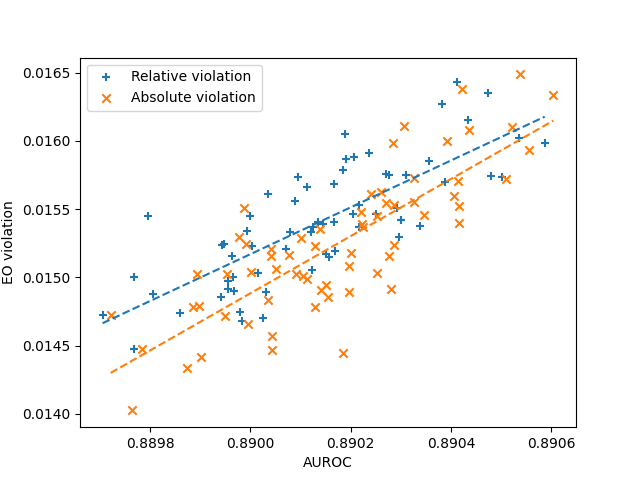
\includegraphics[width=0.9\textwidth]{assets/violations/violation_scatter.png}
\caption{ACSEmployment test score scatter plot of absolute and relative violation each with 75 samples.}
\label{violation_scatter}
\end{figure}



\section{Discussion}

The results provide evidence that the relative violation is less stable during training than the absolute violation. Across the evaluated datasets and fairness metrics, the relative violation consistently resulted in higher variance in the FAIRRET loss. However, the difference in variance was relatively small. This suggests that, although the choice of violation definition affects the stability of the training signal, the magnitude of this effect may be limited in practice.

The results from the model performance experiment provide some indication that this difference in training stability can be reflected in the final fairness of the model. For the ACSEmployment dataset, the absolute violation resulted in a small but statistically significant improvement in the final fairness violation. At the same time, no statistically significant difference in AUROC was observed between the two definitions. This suggests that the increased instability associated with the relative violation does not necessarily result in a substantial loss in predictive performance.

However, these results should not be interpreted as evidence that the relative violation generally produces worse models. The performance experiment was only conducted for one dataset and configuration. Consequently, the observed difference in fairness may be specific to the ACSEmployment dataset, the model architecture, or the particular training configuration used.

An important consideration when interpreting the increased variance is that higher variation in a training loss is not necessarily undesirable. Stochasticity can sometimes be beneficial during optimisation. For example, previous work has investigated deliberately introducing noise or random scaling into optimisation in order to help models escape local minima \todo{TODO: insert reference}. From this perspective, the higher variance produced by the relative violation could potentially have a beneficial effect in some training settings.

There is nevertheless an important distinction between intentional and unintentional sources of variation. If additional variation in the loss is beneficial for optimisation, it can be introduced deliberately through the training procedure, while a variation that arises solely from the choice of fairness definition is not directly controlled. The absolute violation therefore has the advantage of providing a more stable fairness constraint, while any desired stochasticity can still be introduced independently as part of the optimisation procedure.

Overall, the results favour the absolute violation as the more stable definition for use during training. The relative violation produces consistently higher variation in the FAIRRET loss, while the observed performance experiment suggests that this may translate into a small difference in the final fairness achieved. Since the effect on predictive performance was not statistically significant and the performance experiment was limited to a single dataset, the practical advantage of the absolute definition should not be overstated. Nevertheless, when the two definitions are otherwise expected to produce similar results, the greater stability of the absolute violation provides a reason to prefer it as the default definition for model training.